\documentclass[a4paper]{article}


\usepackage[T2A]{fontenc}
\usepackage[utf8]{inputenc}
\usepackage[english,russian]{babel}
\usepackage{graphicx}
\graphicspath{{pictures/}}
\DeclareGraphicsExtensions{.pdf,.png,.jpg}

\usepackage{amsmath, amsfonts, amssymb, amsthm, mathtools}

\author{Шорин Сергей, БКНАД211}
\title{Линейная Алгебра ДЗ 4}
\date{\today}

\begin{document}

\maketitle

\newpage

\section*{1.a}
Переведите из алгебраического вида в тригонометрический: $ -\sqrt{3} + i$

Вынесем число 2($ \sqrt{\sqrt{3}^2 + 1^2} = 2$)

$$2 ( -\frac{\sqrt{3}}{2} + \frac{1}{2}i)$$

Нам подходит угол $\varphi = \frac{5}{6} \pi$

$$ -\sqrt{3} + i = 2(\cos(\frac{5}{6} \pi) + i\sin(\frac{5}{6} \pi)$$



\section*{1.б}
$$-3i$$ \\
Так как здесьб только мнимая часть, то очевидно что угол будет $  + \frac{1}{2}\pi$ или  $  - \frac{1}{2}\pi$\\
Так как аргумент мнимой части отрицательный, то  $\varphi =  - \frac{1}{2}\pi$\\
Найдем модуль: $\sqrt{3^2} = 3$\\
Тогда Ответ:\\
$$-3i = 3*(i\sin(-\frac{1}{2}\pi))$$


\section*{1.в}
$$-1 + i\sqrt{3}$$

Модуль:\\
$\sqrt{1^2 +\sqrt{3}^2}$ = 2\\
тогда получится $ 2(-\frac{1}{2} + i \frac{\sqrt{3}}{2}) = 2(\cos(\frac{2\pi}{3}) + i\sin(\frac{2\pi}{3}))$




\section*{2.a}
Вычислить $\frac{(1 + 3i)(8 - i)}{(2 + i)^ 2}$

$$\frac{(1 + 3i)(8 - i)}{(2 + i)^ 2}= \frac{11 + 23i}{3 + 4i} = \frac{(11 + 23i)(3 - 4i)}{(3 + 4i)(3 - 4i)}= \frac{33 -44i + 69i + 92}{25} = \frac{125 -44i}{25}$$

\section*{2.в}
Вычислить  $\frac{(1 +i)(\sqrt{3} + i)}{(1 - i)(1 - i\sqrt{3})}$\\
$\frac{(1 +i)(\sqrt{3} + i)}{(1 - i)(1 - i\sqrt{3})}$ = $\frac{(1 +i)^2(\sqrt{3} + i)}{(1 +i)(1 - i)(1 - i\sqrt{3})}$ = $\frac{(1 +i)^2(\sqrt{3} + i)}{2(1 - i\sqrt{3})}$ =
 $\frac{(1 +i)^2(\sqrt{3} + i)(1 + i  \sqrt{3})}{2(1 - i\sqrt{3})(1 + i \sqrt{3})}$  =\\
 =  $\frac{(1 +i)^2(\sqrt{3} + i)(1 + i  \sqrt{3})}{2(1 + 3)}$  =   $\frac{(2i)(4i)}{2(1 + 3)}$  = $\frac{-8}{8} $= -1






\section*{3.a}
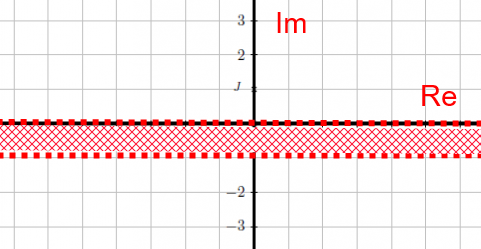
\includegraphics[width=12cm]{1}

\section*{3.б}
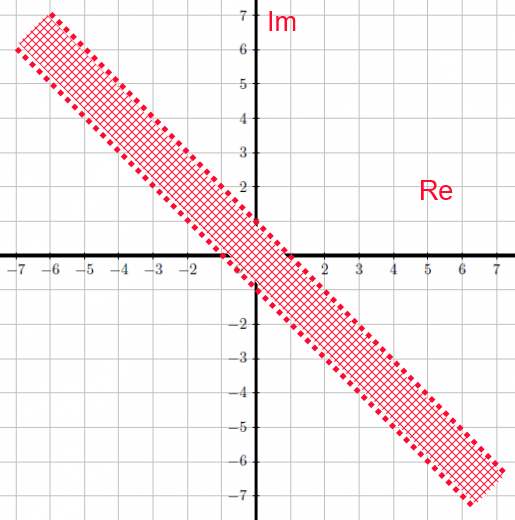
\includegraphics[width=12cm]{2}
\section*{3.в}
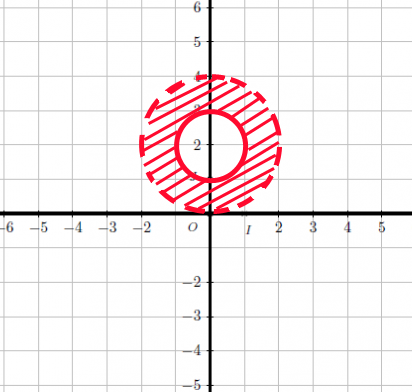
\includegraphics[width=12cm]{3}
\section*{4.a}
Вычислите, применив формулу Муавра: $(1 + i \sqrt{3})^{150}$

Переведем в тригонометрический вид:

$$(1 + i \sqrt{3})^{150} = 2^{150}(\cos(\frac{\pi}{3}) + i\sin(\frac{\pi}{3}))^{150} = 2^{150}(\cos(50\pi) + i\sin(50\pi)) = 2^{150}$$


\section*{4.б}

Вычислите, применив формулу Муавра:
$$(\frac{\sqrt{3} + i}{1 -i})^{30}=
(\frac{2(\cos(\frac{\pi}{6}) + i\sin(\frac{\pi}{6}))}{\sqrt{2}(\cos(\frac{-\pi}{4}) + i\sin(\frac{-\pi}{4}))})^{30} 
$$
$$
(\frac{2(\cos(\frac{\pi}{6}) + i\sin(\frac{\pi}{6}))}{\sqrt{2}(\cos(\frac{-\pi}{4}) + i\sin(\frac{-\pi}{4}))})^{30}  = \frac{2^{15}(\cos(\frac{\pi}{6}) + i\sin(\frac{\pi}{6}))^{30}}{(\cos(\frac{-\pi}{4}) + i\sin(\frac{-\pi}{4}))^{30}}=
\frac{2^{15}(\cos(30\frac{\pi}{6}) + i\sin(30\frac{\pi}{6}))}{(\cos(30\frac{-\pi}{4}) + i\sin(30\frac{-\pi}{4}))}
=$$
$$ 
=
\frac{2^{15}(\cos(\pi) + i\sin(\pi)}{(\cos(\frac{-3\pi}{2}) + i\sin(\frac{-3\pi}{2}))}=
2^{15}\cos(\pi - \frac{-3\pi}{2}) + i\sin(\pi - \frac{-3\pi}{2})=
2^{15}\cos(\frac{\pi}{2}) + i\sin(\frac{\pi}{2})=
$$
$$
= 2^{15}\cos(\frac{\pi}{2}) + i\sin(\frac{\pi}{2}) = 2^{15}i
$$

\section*{5.а}
Вычислить $\sqrt[3]{8}$
$$\sqrt[3]{8} = 2$$

\section*{5.б}
Вычислить $\sqrt[8]{2\sqrt{2}(1 - i)}$
$$\sqrt[8]{2\sqrt{2}(1 - i)} = \sqrt[8]{4(\frac{1}{\sqrt{2}} - i\frac{1}{\sqrt{2}})} = \sqrt[8]{4(\cos(-\frac{\pi}{4}) - i\sin(-\frac{\pi}{4}))}$$
$$\sqrt[8]{4(\cos(-\frac{\pi}{4}) - i\sin(-\frac{\pi}{4}))} =\sqrt[4]{2} (\cos(\frac{(-\frac{\pi}{4} + 2 \pi k)}{8}) - i\sin(\frac{(-\frac{\pi}{4} + 2 \pi k)}{8})), k \in [0, 7] $$

\section*{6.a}
Решить квадратное уравнение $x^2 - 4x	 + 29$


$$x_1, x_2 = \frac{4 \pm \sqrt{16-  4 * 29}}{2} = 2 \pm 5 \sqrt{-1} = 2 \pm 5 i$$
\section*{6.б}
Решить квадратное уравнение $x^2 - x	 + 1 + i$


$$x_1, x_2 = \frac{1 \pm \sqrt{1 -  4 - 4i}}{2} =\frac{1 \pm \sqrt{-3 - 4i}}{2} = \frac{1 \pm i\sqrt{3 + 4i}}{2} = \frac{1 \pm i\sqrt{(2 + i)^2}}{2}= $$
$$=\frac{1 \pm i(2 + i)}{2} =\frac{1 \pm (2i - 1)}{2} $$

$$x_1 = \frac{2i}{2} = i$$
$$x_2 = \frac{2 - 2i}{2} = 1- i$$

\end{document}